\section{User Interface Design}
\subsection{User Experience}
\subsubsection{Traditional User}
This is the UX from the point of view of a customer. From the homepage he can perform a request as a guest, adding some basic personal information and giving the consensus of using his position. He can also register to the service, compiling a registration form, or login in if already registered. Both choices lead to a new page in which the now registered passenger can perform requests without adding any extra information or reservations, filling the corresponding form.
\begin{figure}[h!]
	\begin{center}
		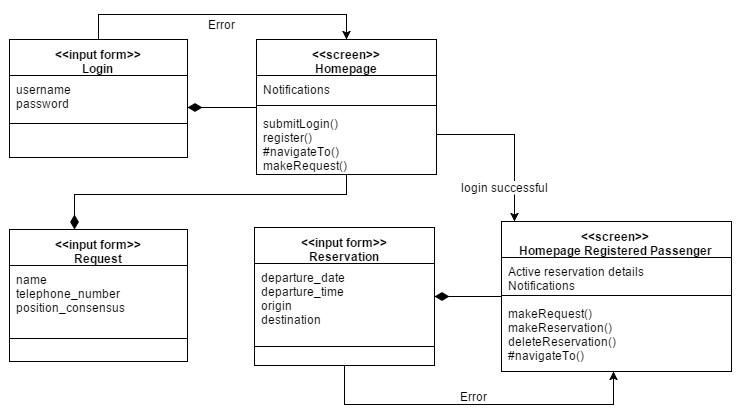
\includegraphics[width=1\linewidth]{../SE2_IMAGES/UserUX}
		\caption{User Experience - User}
	\end{center}
\end{figure}
\newpage
\subsubsection{Taxi Driver}
This is the UX from the point of view of a taxi driver. From the homepage he still is considered a guest so he has access to the same functionalities that we have explained for the UX above. Once loggend in he has a completely different interface with respect to the customer. He can set his status as available or unavailable, see if there is a pending request and in case accept or refuse it.
\begin{figure}[h!]
	\begin{center}
		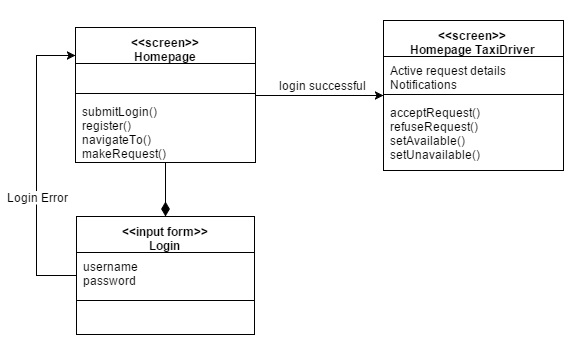
\includegraphics[width=1\linewidth]{../SE2_IMAGES/TaxiUX}
		\caption{User Experience - Taxi Driver}
	\end{center}
\end{figure}